% BOTTOM caption
% ------------------------
\begin{figure}[!htbp]
\centering
\vspace{1\baselineskip}
% ------------------------
%
% Main information
% ===========================================================
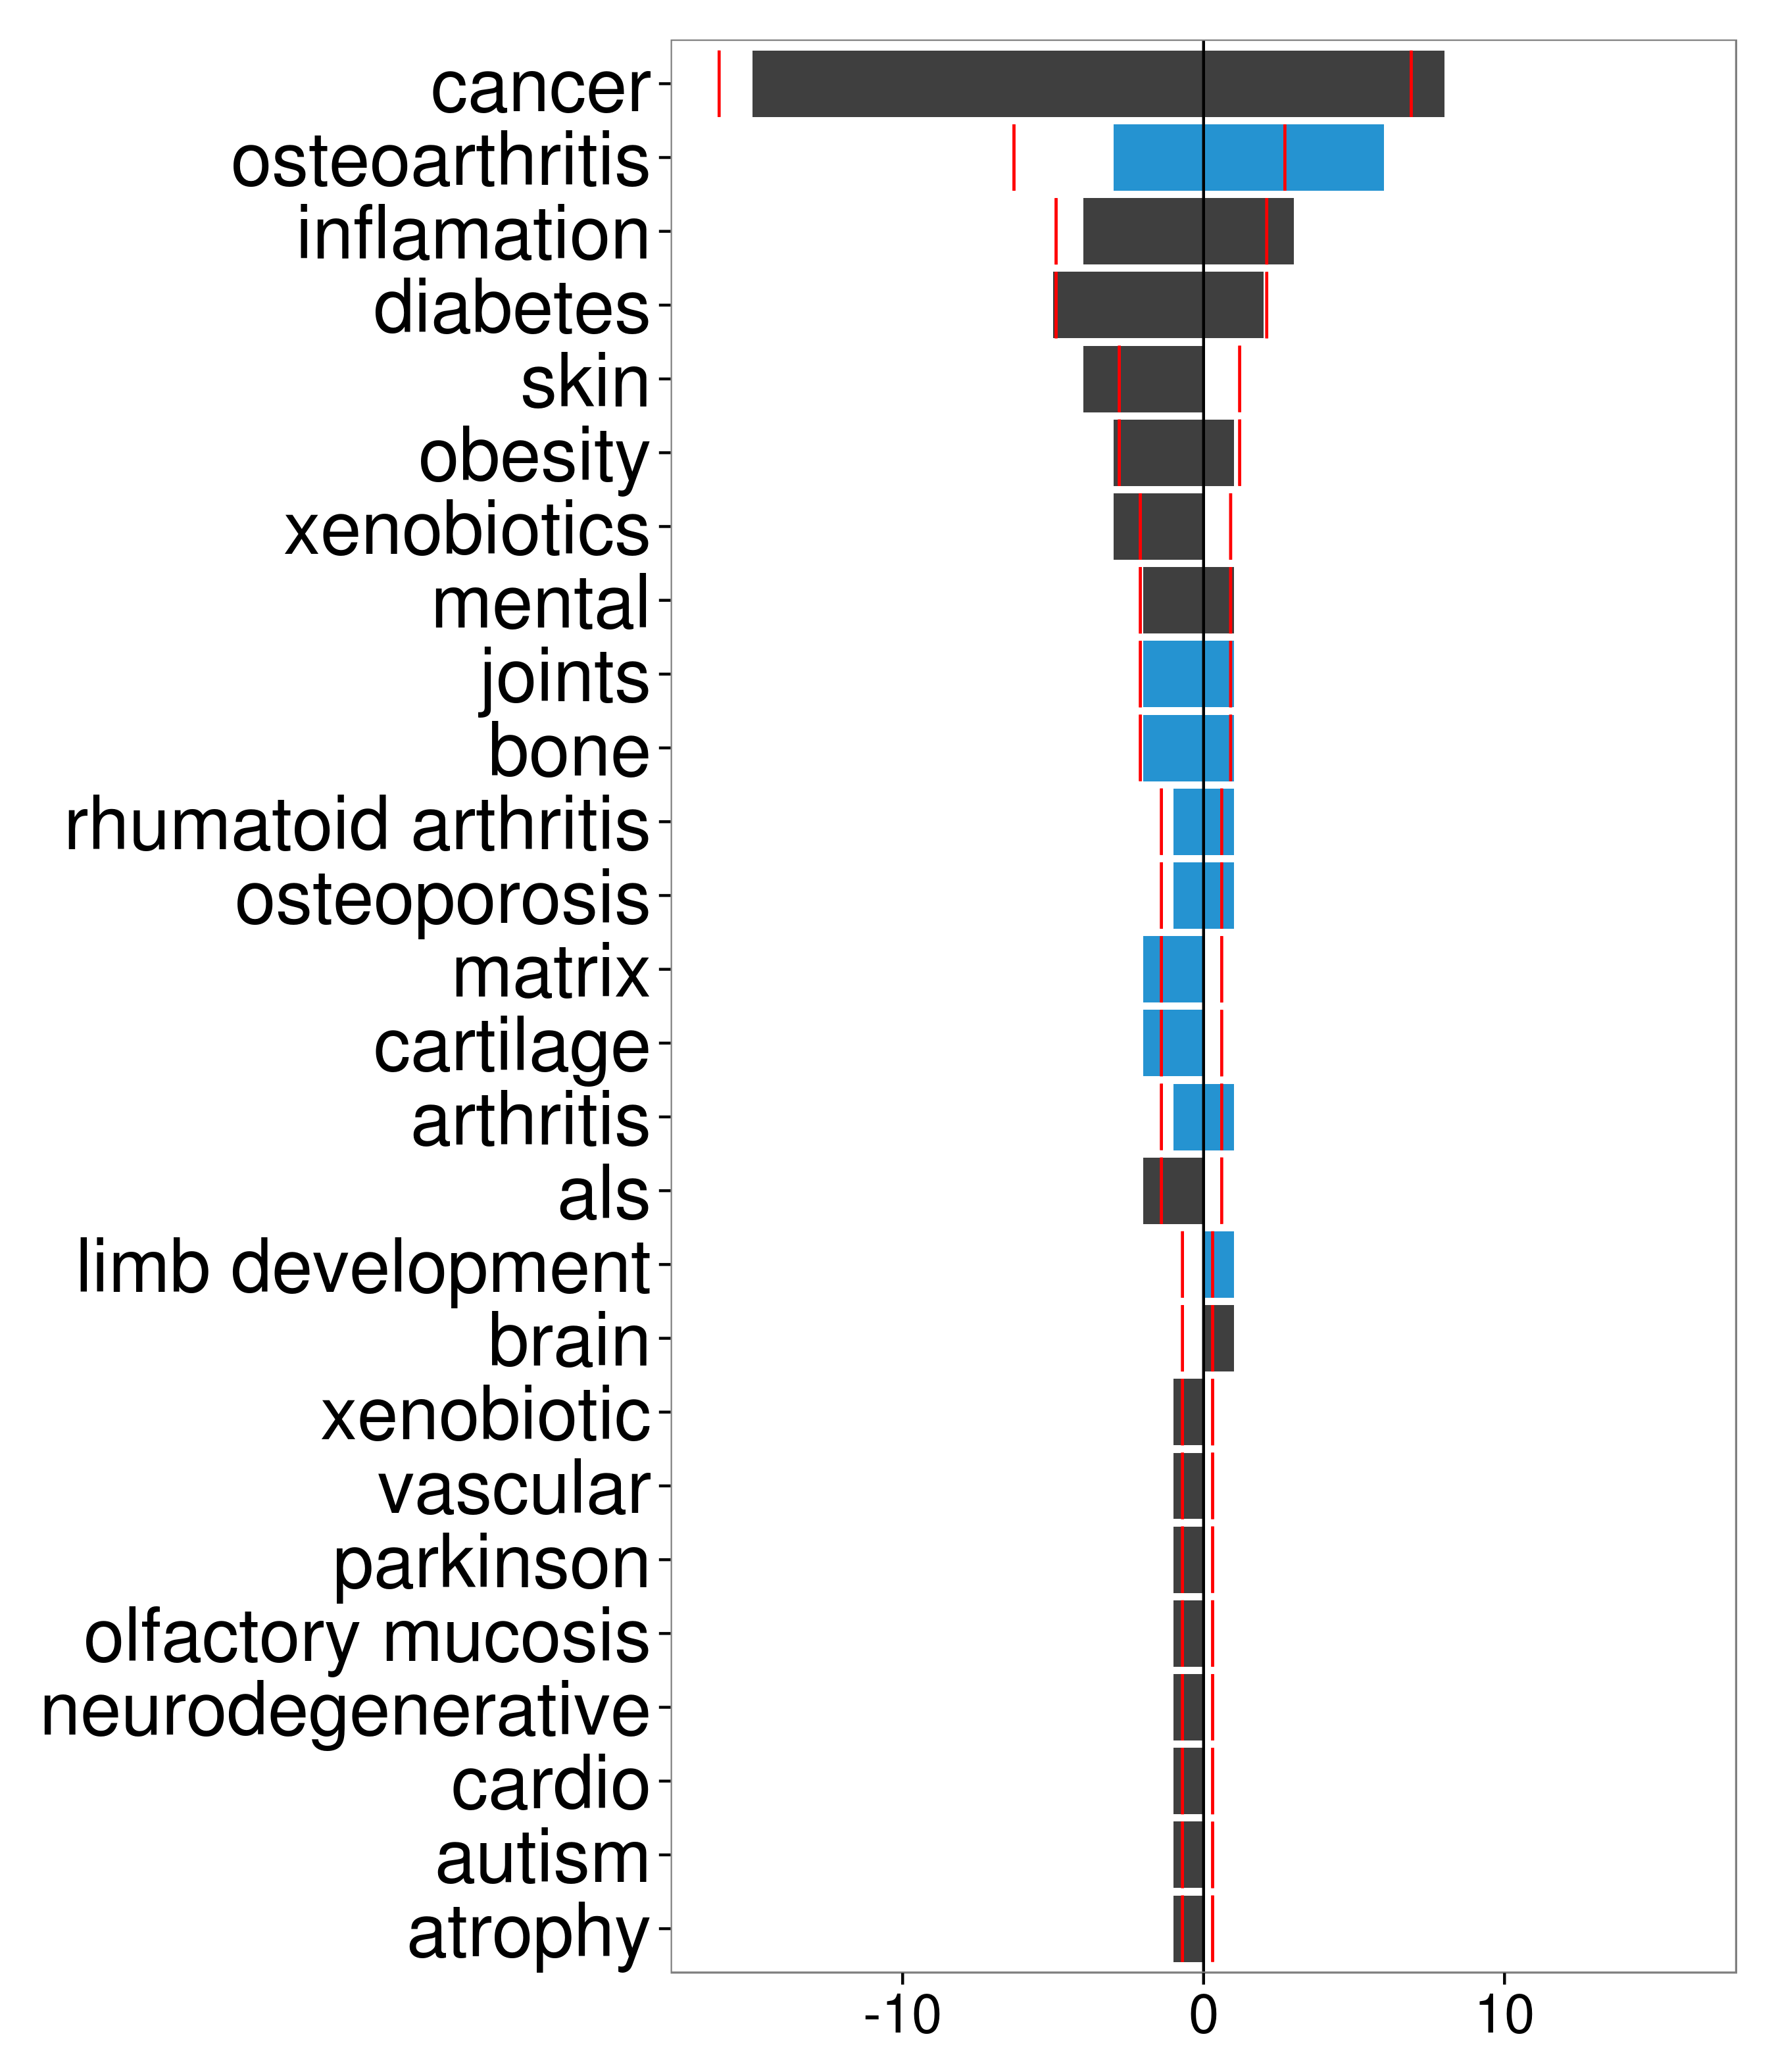
\includegraphics[width=0.8\textwidth]
{Figures/hlc-manualannot-antago/hlc-manualannot-antago.png}
\caption[Catégories fonctionnelles enrichies parmi les gènes "antagonisés" dans les bourgeons de membres postérieurs]
{
Catégories fonctionnelles enrichies parmi les gènes présentant un profil d'"antagonisation" et réprimés (valeurs négatives, partie gauche de chaque sous-figure) ou induits (valeurs positives, partie droite de chaque sous-figure) dans les \glspl{hlb}.
La valeur absolue de l'axe des abscisses représente le nombre de gène associé à chaque terme (axe des ordonnées).
Les barres verticales rouge correspondent au nombre théorique de gènes associés à chaque terme dans le cas d'une répartition aléatoire entre répression et induction.
Les termes bleus sont associés au squelette.
}
\label{fig:hlc-manualannot-antago}
% ===========================================================
%
% BOTTOM caption
% ------------------------
\end{figure}
% ------------------------